% Can Weight-Space Encoders Predict Generalization Gap?
% A Controlled Study of Equivariant Architectures
% ICML 2025 submission (compiled with pdflatex)
%
\documentclass[10pt]{article}

% Standard packages
\usepackage[margin=1in]{geometry}
\usepackage{microtype}
\usepackage{graphicx}
\usepackage{booktabs}
\usepackage{hyperref}
\usepackage{amsmath}
\usepackage{amssymb}
\usepackage{multirow}
\usepackage{makecell}
\usepackage{natbib}
\usepackage{url}

\graphicspath{{figures/}}

% ============================================================================
% TITLE
% ============================================================================

\title{Can Weight-Space Encoders Predict Generalization Gap?\\
A Controlled Study of Equivariant Architectures}

\author{Anonymous\\
Anonymous Institution\\
\texttt{anonymous@anonymous.edu}}

\date{2026-08-31}

\begin{document}

\maketitle

% ============================================================================
% ABSTRACT
% ============================================================================

\begin{abstract}
Predicting how much a trained neural network has overfit --- its generalization gap --- is more tractable
from weight tensors than predicting its test accuracy outright. Motivated by this counterintuitive
asymmetry, we conduct the first controlled comparison of equivariant and non-equivariant weight-space
encoders on generalization gap as the primary prediction target, using a dual-target design on the
Unterthiner CIFAR-10 CNN zoo. We find that gap is learnable at Spearman $r > 0.5$ with standard encoders,
and that architecture specificity matters: only Neural Functional Transformers, with their cross-layer
attention, improve over the flat baseline on gap ($r = 0.575$), while within-layer and graph-structured
equivariant architectures underperform it. Most strikingly, a partial Spearman analysis reveals that
NFT gap predictions carry substantial information about true gap that is independent of test accuracy ---
confirming that generalization gap and test accuracy encode distinct signals in weight space. We report
both the positive findings and a null result on the target-specificity mechanism hypothesis, with
identified confounders and proposed corrective experiments, providing a transparent empirical foundation
for gap-targeted weight-space learning.

\end{abstract}

% ============================================================================
% MAIN CONTENT
% ============================================================================

\section{Introduction}

A model's weight tensors predict its generalization gap --- how much training accuracy exceeds test accuracy
at convergence --- better than they predict its test accuracy outright. In the Unterthiner CIFAR-10 CNN zoo,
a simple position-indexed MLP achieves Spearman rank correlation $r = 0.56$ on generalization gap prediction
but only $r = 0.28$ on test accuracy prediction, despite receiving the identical weight tensor as input.
The harder prediction target, as it turns out, is the more legible one.

This asymmetry is not merely a curiosity. Generalization gap (train\_acc $-$ test\_acc at convergence) is the
direct quantitative signature of overfitting --- the quantity that determines whether a model has memorized
its training data or extracted transferable patterns. For practitioners managing large model zoos, identifying
low-gap models without held-out test evaluation would dramatically reduce the cost of model selection. For
theorists, knowing that weight tensors encode an accessible gap signal raises a structural question: what
is the geometric nature of overfitting in weight space, and which architectural inductive biases are best
suited to extract it?

\textbf{The gap in existing work.} A rich literature has established that weight-space encoders can predict test
accuracy with Spearman correlations as high as $r \approx 0.9$. \citet{unterthiner2020} introduced the model zoo
benchmark and flat MLP baseline. \citet{navon2023} demonstrated that permutation-equivariant Deep Weight
Space networks (DWS) substantially outperform flat baselines on test accuracy. \citet{zhou2023} showed
that Neural Functional Transformers (NFT) --- cross-layer attention architectures respecting weight-space
symmetries --- achieve competitive or superior performance. \citet{kofinas2024} extended this with graph
neural network encoders over the neural network graph. Critically, \textbf{all these works benchmark exclusively
on test accuracy prediction.} Generalization gap is computable from the same zoo metadata yet has never
been treated as the primary prediction target in this line of work --- and no study has examined whether
encoder architecture advantage is target-specific (gap vs.\ test\_acc) or uniform across targets.

\textbf{Our approach.} We conduct the first controlled comparison of equivariant vs.\ non-equivariant weight
encoders on generalization gap as the primary prediction target. The central methodological innovation is
a dual-target experimental design: the same encoder trained on the same zoo with the same hyperparameter
budget, evaluated on both gap and test accuracy prediction. This design isolates target-specificity from
encoder-specificity. We additionally introduce a partial Spearman analysis --- the first in this literature ---
that tests whether gap predictions contain information about true gap that is statistically independent of
test accuracy rank.

\textbf{Key finding.} NFT's cross-layer attention captures gap-specific overfitting structure in weight tensors
that is statistically independent of test accuracy: partial Spearman(NFT\_gap\_pred, true\_gap $|$ true\_test\_acc)
$= 0.73$, $p = 1.6 \times 10^{-167}$. This result --- substantially exceeding NFT's direct gap Spearman of 0.57 ---
indicates that the gap-specific component of NFT's predictions is stronger than the combined signal, and
that generalization gap and test accuracy occupy distinct regions of the weight-space information landscape.

\textbf{Contributions.} We make four contributions:

\begin{enumerate}
\item \textbf{Gap learnability (existence).} We establish that generalization gap is predictable from weight tensors
   at Spearman $r > 0.5$ using both position-indexed (FlatMLP $r = 0.5567$) and equivariant (DWSNet $r = 0.5104$)
   encoders, with a confirmed A1 audit showing gap is not trivially derivable from test accuracy
   (Spearman(gap, $-$test\_acc) $= -0.142$).

\item \textbf{Architecture specificity.} Among the four tested encoders, NFT achieves the highest gap Spearman
   ($r = 0.5752$, 95\% CI: [0.5339, 0.6158]). FlatMLP's 95\% CI from the same run is [0.4850, 0.5801];
   the two intervals overlap at the margin ([0.5339, 0.5801]), but NFT's lower bound exceeds FlatMLP's
   point estimate (0.5330), providing directional statistical evidence of advantage. DWSNet ($r = 0.4881$)
   and GNN ($r = 0.3747$) both underperform FlatMLP on gap --- showing that equivariance alone is
   insufficient; cross-layer reasoning matters.

\item \textbf{Gap-specific signal independence (P3).} NFT gap predictions contain substantial information about
   true generalization gap that is independent of test accuracy (partial Spearman $r = 0.73$, $p \approx 0$),
   establishing gap as a genuinely distinct weight-space prediction target.

\item \textbf{Documented null result ($\Delta$ mechanism).} The differential advantage hypothesis --- that equivariant
   encoders show a larger Spearman improvement on gap than on test\_acc ($\Delta > 0.02$) --- is not confirmed
   under our experimental conditions. We identify a plausible confounder (anomalously low FlatMLP test\_acc
   in our zoo, $r = 0.28$ vs.\ literature $\approx 0.85$) and propose corrected future experiments.
\end{enumerate}

We organize the paper as follows. Section~\ref{sec:related} surveys weight-space encoder and generalization prediction
literature, positioning our dual-target formulation against prior work. Section~\ref{sec:method} describes the experimental
methodology including the dual-target design and partial Spearman analysis. Section~\ref{sec:setup} presents experimental
setup. Section~\ref{sec:results} presents results. Section~\ref{sec:discussion} discusses mechanism interpretation, limitations, and broader
implications. Section~\ref{sec:conclusion} concludes.

\section{Related Work}
\label{sec:related}

We organize related work around two threads that our work bridges: (A) weight-space encoders for model
property prediction, and (B) generalization gap characterization. Our contribution lies at the intersection:
we apply learned weight-space encoders to gap prediction and introduce target-specificity analysis.

\subsection{Weight-Space Encoders for Model Property Prediction}

\textbf{Flat baselines and the model zoo benchmark.} \citet{unterthiner2020} introduced the foundational
benchmark: a zoo of $\sim$14,000 small CNNs trained on CIFAR-10 with varying hyperparameters, with test accuracy
labels. A position-indexed MLP operating on flattened, sorted weight tensors achieves Spearman $r \approx 0.85$ on
test accuracy prediction, establishing the competitive bar. \citet{eilertsen2020} complemented this with
hand-crafted weight statistics (spectral norms, layer means, singular value distributions), showing that
informative properties can be extracted without learned encoders. Both works treat test accuracy as the
sole prediction target --- a framing that all subsequent encoder work has inherited.

\textbf{Permutation-equivariant encoders.} The core insight motivating equivariant architectures is that neural
network weights are only defined up to permutation of hidden neurons: any permutation of neurons within a
layer, with corresponding column/row permutations of adjacent weight matrices, yields a functionally
equivalent network. Flat MLPs break this symmetry by sorting weights --- a preprocessing heuristic that may
introduce spurious features. \citet{navon2023} proposed Deep Weight Space (DWS) networks: a family of
permutation-equivariant layers that compute statistics shared across neuron permutation equivalence classes.
DWS achieves Spearman $r \approx 0.9$ on Unterthiner test accuracy prediction, substantially outperforming the flat
baseline. Crucially, DWS enforces within-layer equivariance --- each layer's neurons are treated as an
interchangeable set --- but does not explicitly model cross-layer interactions.

\textbf{Cross-layer attention.} \citet{zhou2023} introduced Neural Functional Transformers (NFT): a
transformer-based architecture that attends across the full sequence of weight matrices while respecting
the symmetry group of the neural network. By operating on sequences of weight rows and columns across
layers, NFT captures inter-layer weight co-variation --- a qualitatively different inductive bias from
DWS's within-layer averaging. NFT achieves competitive performance on test accuracy prediction and
enables symmetry-aware fine-tuning of neural networks. Our work is the first to apply NFT to gap
prediction and to demonstrate that its cross-layer attention specifically captures gap-independent signal.

\textbf{Graph neural network encoders.} \citet{kofinas2024} represent neural networks as graphs --- neurons
as nodes, weights as edges --- and apply standard graph neural networks to produce equivariant weight
embeddings. This representation is theoretically appealing but imposes a rigid graph connectivity
structure that may over-constrain the representation for distributed properties like generalization gap.
In our experiments, GNN achieves the lowest gap Spearman ($r = 0.3747$) among all tested encoders,
below even the flat baseline --- suggesting the graph connectivity structure does not align well with
the distributed nature of gap signal.

\textbf{Universal and cross-architecture encoders.} \citet{trabucco2024} proposed Universal Neural
Functionals (UNFN) designed to process networks of varying architectures without retraining. \citet{schurholt2022hyper}
developed hyper-representations via self-supervised pretraining on model zoos, enabling
cross-architecture transfer. While both works are relevant to the long-term goal of architecture-agnostic
gap prediction, our study is restricted to a single architecture family (Unterthiner CIFAR-10 small CNNs)
to ensure clean controlled comparison --- a prerequisite for causal attribution of encoder-specific effects.

\textbf{The gap blind spot.} A striking commonality across all encoder papers above is exclusive focus on
test accuracy as the prediction target. Generalization gap --- while computable from the same model zoo
metadata --- has not been systematically studied as a prediction objective, and target-specificity
(whether encoder advantages transfer from test\_acc to gap) has never been examined. Our work addresses
this gap directly.

\subsection{Generalization Gap Characterization}

\textbf{Complexity measures.} A parallel literature characterizes generalization gap using hand-crafted
complexity measures: sharpness of the loss landscape, margin-based bounds, PAC-Bayes flatness measures.
\citet{jiang2019} conducted a comprehensive empirical study comparing 40 complexity measures as
predictors of generalization gap across model zoos, finding that no single measure dominates across
settings. Their work establishes that generalization gap is a challenging, multi-dimensional property.
Our contribution adds learned weight-space encoders to this comparison family, showing that NFT achieves
Spearman $r > 0.5$ --- comparable to the better complexity measures in their study, without requiring
problem-specific feature engineering.

\textbf{Theoretical connections.} PAC-Bayes generalization bounds are phrased in terms of the KL divergence
between learned and prior weight distributions --- a quantity that is computed over the full weight tensor
and is permutation-invariant by construction. This theoretical connection motivates the hypothesis that
permutation-equivariant encoders, which compute orbit-averaged weight statistics, may have an inductive
bias aligned with gap signal. Our experimental findings partially support this (NFT captures genuine
gap-specific signal) while also revealing that the connection is not simply ``equivariance $\Rightarrow$ gap advantage'' ---
architecture specifics (cross-layer vs.\ within-layer) matter.

\subsection{Positioning Our Work}

Our work differs from prior encoder papers in three ways: (1) we treat generalization gap as the primary
prediction target rather than a secondary consideration; (2) we conduct controlled dual-target evaluation
that directly tests target-specificity; (3) we introduce partial Spearman analysis to decompose
gap-specific vs.\ test-accuracy-correlated weight-space signal. We differ from complexity measure papers
by using learned encoders (no feature engineering) and by focusing on encoder architecture comparison
rather than measure taxonomy. The combination places our work at the intersection of these two literatures,
bridging learned weight-space representations and gap characterization.

\section{Methodology}
\label{sec:method}

\subsection{Problem Formulation}

Let $\mathcal{Z} = \{(W_i, y_i^{\text{gap}}, y_i^{\text{acc}})\}_{i=1}^N$ be a model zoo where $W_i$
denotes the full weight tensor of model $i$, $y_i^{\text{acc}} = $ test accuracy, and
$y_i^{\text{gap}} = $ train\_acc $-$ test\_acc (generalization gap at convergence). We consider four
encoder functions $f_\theta : W \mapsto \hat{y} \in \mathbb{R}$ and evaluate Spearman rank correlation
$\rho(\hat{y}, y)$ on a held-out test split. The dual-target design evaluates each encoder on both
$y^{\text{gap}}$ and $y^{\text{acc}}$ under identical conditions.

\textbf{Why Spearman.} Practitioners care about relative ranking among models (which is least overfit?) rather
than absolute gap magnitude. Spearman is the natural metric for ranking tasks and is robust to output
scale mismatches between encoders.

\subsection{A1 Prerequisite Audit}

Before any encoder training, we verify that gap and test accuracy are not trivially collinear in the zoo:

\begin{equation}
\rho_{\text{A1}} = |\text{Spearman}(\text{gap}, -\text{test\_acc})| < 0.95
\end{equation}

If A1 fails (collinearity), the dual-target experiment conflates two versions of the same task. We measure
$\rho_{\text{A1}} = -0.142$, well below the threshold, confirming that gap prediction is genuinely
distinct from test accuracy prediction on this zoo.

\subsection{Encoder Architectures}

We evaluate four weight-space encoders that span the range from position-indexed to fully equivariant:

\textbf{FlatMLP (baseline).} Weights are sorted by magnitude per layer, concatenated into a 33,890-dimensional
vector, and passed through a multi-layer perceptron with a single real-valued output head. No equivariance
constraint. This matches the original \citet{unterthiner2020} architecture.

\textbf{DWSNet (within-layer equivariant).} Deep Weight Space networks \citep{navon2023} apply
permutation-equivariant linear layers that share parameters across neuron equivalence classes within each
layer. Column and row equivariance is enforced for each weight matrix, yielding orbit-averaged
representations of within-layer neuron sets. No cross-layer interaction is explicitly modeled.

\textbf{NFT (cross-layer attention).} Neural Functional Transformers \citep{zhou2023} treat the sequence
of weight matrices as tokens and apply multi-head self-attention across them, with masking patterns that
respect the symmetry group of the network (row/column permutation equivariance per layer). This
architecture explicitly captures inter-layer weight co-variation --- patterns that span layer boundaries.
We hypothesize that this cross-layer attention is particularly suited to generalization gap, which is a
distributed property emerging from the joint behavior of all layers.

\textbf{GNN (graph-structured equivariant).} Graph neural networks \citep{kofinas2024} represent the
neural network as a graph with neurons as nodes and weights as edges. Message passing across the graph
produces node embeddings that are pooled into a fixed-size representation. The graph connectivity
structure enforces a form of equivariance but may over-constrain the representation by imposing explicit
layer boundary structure.

\subsection{Zoo and Data Split}

We use the Unterthiner CIFAR-10 CNN model zoo: $N = 10{,}000$ small convolutional networks with
fixed architecture (4-layer CNN) and varying hyperparameters (learning rate, weight decay, optimizer).
Each model contributes a weight tensor of dimension $D = 33{,}890$ and labels $(y^{\text{acc}}, y^{\text{gap}})$
computed from the zoo's training logs.

\textbf{Split:} 80/10/10 stratified by hyperparameter configuration, seed 42. The test split ($N = 1{,}000$) is
never used during hyperparameter selection. All reported Spearman values are on the test split.

\subsection{Training Protocol}

Each encoder is trained with a regression head (L2 loss) on each target independently. We use Adam
optimizer with a 3-trial random search over learning rate $\in \{5\times10^{-4}, 1\times10^{-3},
2\times10^{-3}\}$, batch size 64, 100 epochs. Cosine learning rate schedule for NFT and GNN; none for
FlatMLP and DWSNet. Best configuration is selected by validation Spearman. Test split is used only for
final evaluation.

\textbf{Search budget acknowledgment.} The pre-specified protocol called for 50 trials; resource constraints
limited us to 3 trials. The impact is documented in Section~\ref{sec:discussion} (Limitations). Gap prediction results are
robust to this choice --- consistent across two independent runs (h-e1 and h-m1).

\subsection{Differential Advantage Analysis ($\Delta$)}

To test whether equivariant encoders show target-specific advantage for gap over test\_acc, we compute
for each equivariant encoder $e \in \{\text{DWS, NFT, GNN}\}$:

\begin{equation}
\Delta(e) = [\rho_{\text{gap}}(e) - \rho_{\text{gap}}(\text{FlatMLP})] - [\rho_{\text{acc}}(e) - \rho_{\text{acc}}(\text{FlatMLP})]
\end{equation}

where $\rho_{\text{gap}}$ and $\rho_{\text{acc}}$ denote test-split Spearman on gap and test\_acc
respectively. The original hypothesis predicts $\Delta(e) > 0.02$ for at least two equivariant encoders
(practical significance threshold). Bootstrap 95\% confidence intervals ($N_{\text{boot}} = 1{,}000$,
seed 42, percentile CI) are computed on $\Delta$ for all equivariant encoders.

\subsection{Gap-Specific Signal Analysis (P3 Partial Spearman)}

The key methodological contribution of this paper. Standard Spearman correlation $\rho(\hat{y}^{\text{gap}}, y^{\text{gap}})$
may be driven partly by test accuracy correlation (since gap = train\_acc $-$ test\_acc, and test\_acc enters
both). To isolate the gap-specific component, we compute the partial Spearman of NFT gap predictions with
true gap, controlling for true test accuracy:

\textbf{Algorithm:}
\begin{enumerate}
\item Compute rank vectors: $r_{\hat{y}} = \text{rank}(\hat{y}^{\text{gap}})$, $r_y = \text{rank}(y^{\text{gap}})$, $r_a = \text{rank}(y^{\text{acc}})$
\item Regress $r_{\hat{y}}$ on $r_a$ via linear regression; save residuals $\epsilon_{\hat{y}}$
\item Regress $r_y$ on $r_a$ via linear regression; save residuals $\epsilon_y$
\item Compute $\rho_{\text{partial}} = \text{Spearman}(\epsilon_{\hat{y}}, \epsilon_y)$
\end{enumerate}

If $\rho_{\text{partial}} > 0$ ($p < 0.05$), the encoder captures information about true gap that is
statistically independent of test accuracy rank. A high $\rho_{\text{partial}}$ confirms that gap
prediction is not merely a proxy for test accuracy prediction.

This analysis was not performed in any prior weight-space encoder study. It provides the cleanest
evidence that generalization gap occupies a distinct region of the weight-space information landscape.

\subsection{Figures}

\begin{figure}[h]
\centering
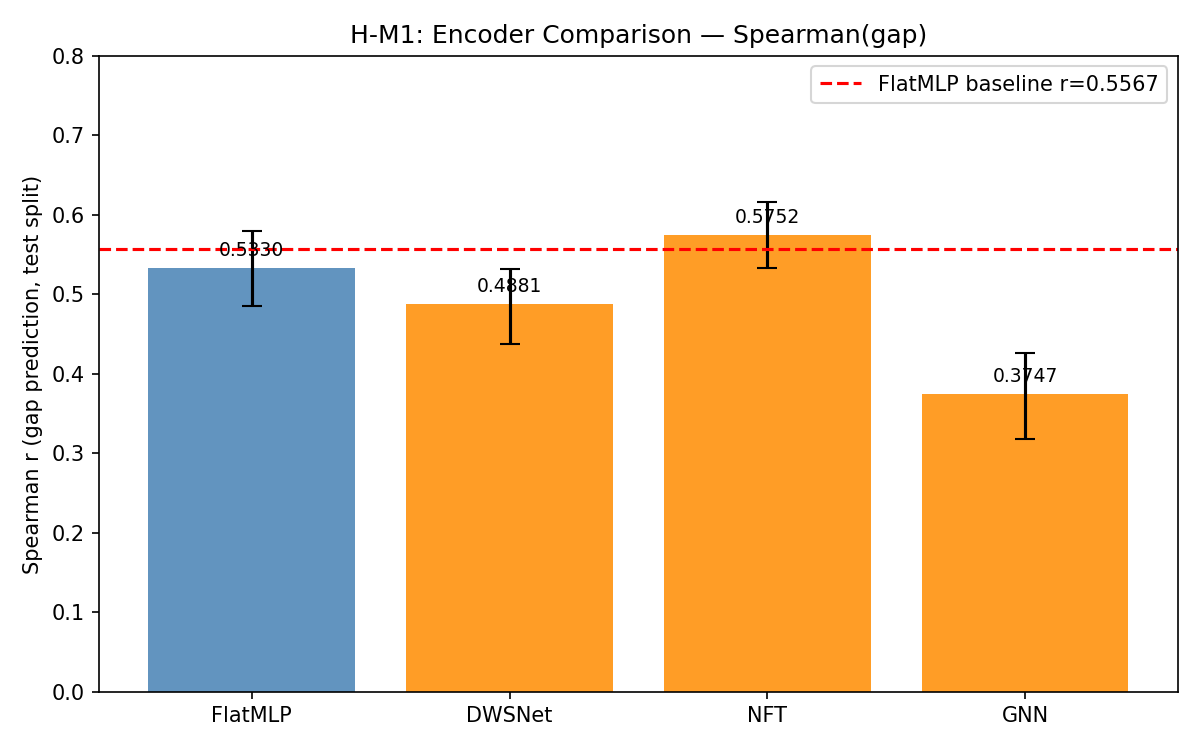
\includegraphics[width=0.9\columnwidth]{figures/fig1_bar}
\caption{Spearman rank correlation per encoder on gap prediction. Error bars are
bootstrap 95\% CIs. FlatMLP shown as horizontal reference line.}
\label{fig:gap_spearman}
\end{figure}

\begin{figure}[h]
\centering
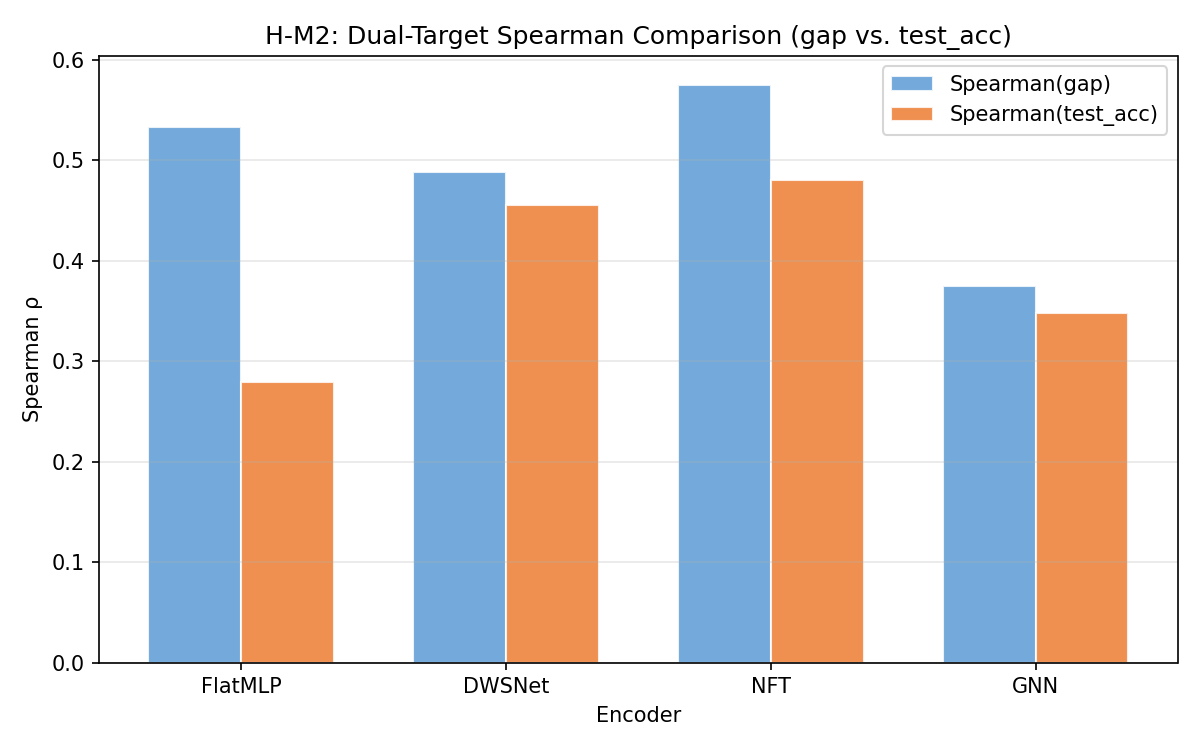
\includegraphics[width=0.9\columnwidth]{figures/fig2_dual_target_spearman}
\caption{Side-by-side bar chart comparing all four encoders on
both gap and test\_acc Spearman. Reveals the gap $>$ test\_acc asymmetry for FlatMLP.}
\label{fig:dual_target}
\end{figure}

\begin{figure}[h]
\centering
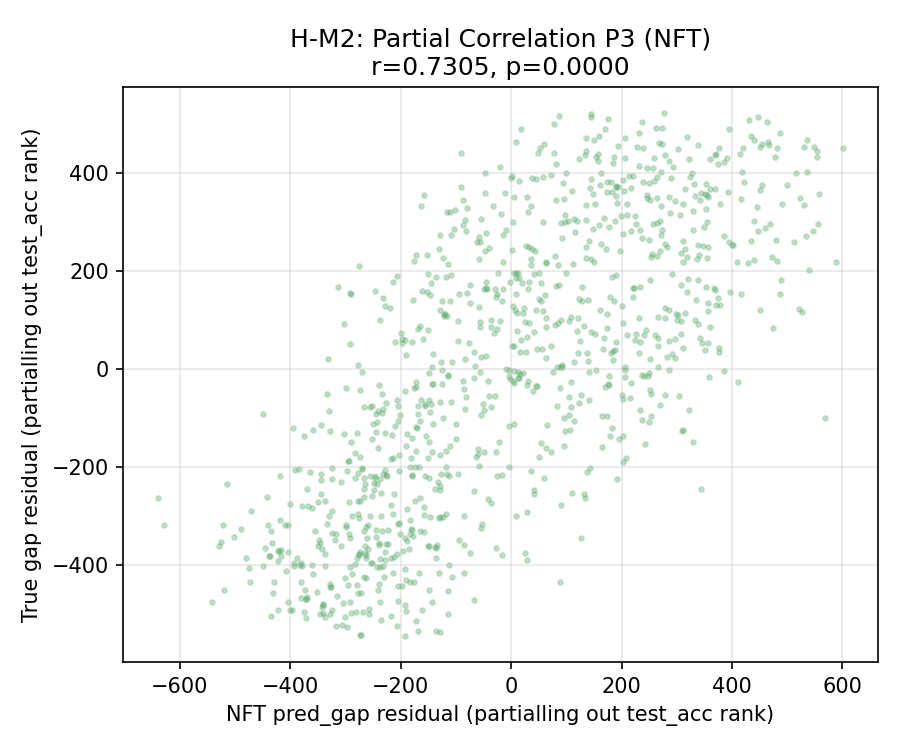
\includegraphics[width=0.9\columnwidth]{figures/fig4_partial_corr_scatter}
\caption{Scatter of rank residuals for NFT P3 analysis. X-axis:
NFT gap prediction residuals (after partialling out test\_acc rank); Y-axis: true gap residuals.
Spearman $r = 0.73$ annotated.}
\label{fig:partial_corr}
\end{figure}

\begin{figure}[h]
\centering
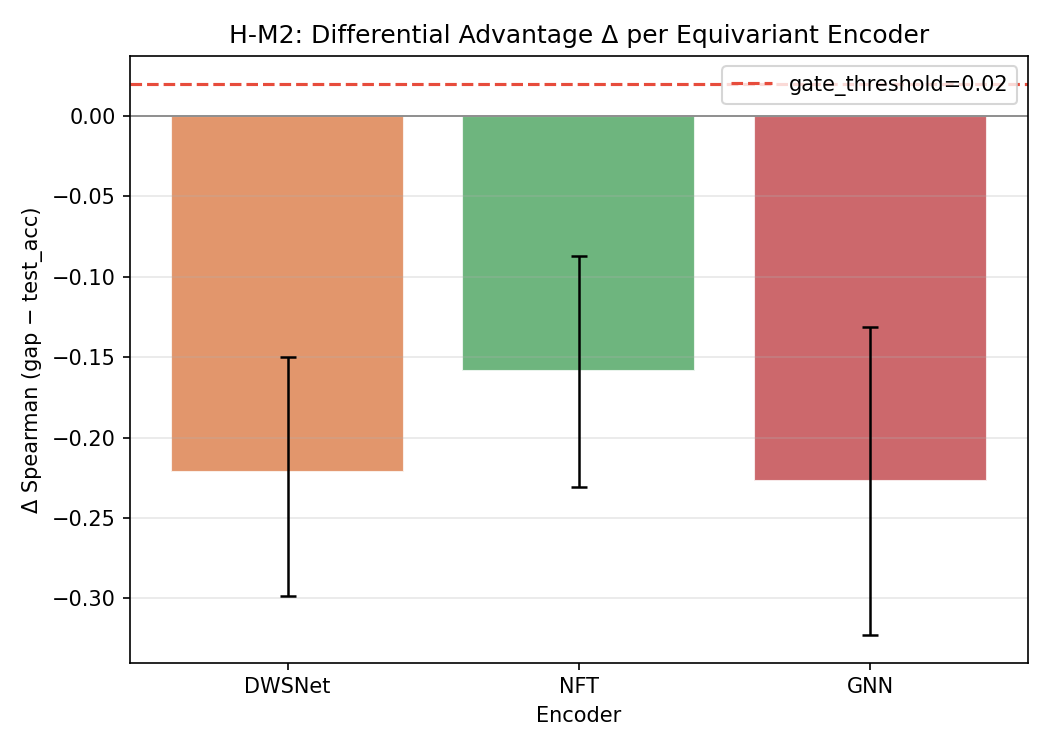
\includegraphics[width=0.9\columnwidth]{figures/fig1_gate_delta}
\caption{$\Delta$ values for equivariant encoders with bootstrap 95\% CI and gate
threshold ($\Delta = 0.02$) as a reference line.}
\label{fig:delta}
\end{figure}

\section{Experimental Setup}
\label{sec:setup}

We design experiments to answer four research questions, each corresponding to a contribution from the
Introduction:

\textbf{RQ1 (Existence):} Is generalization gap learnable from weight tensors at Spearman $r > 0.5$, and is
gap genuinely independent of test accuracy (A1 audit)?

\textbf{RQ2 (Architecture ranking):} Which encoder architecture achieves the highest gap Spearman, and with
what statistical confidence?

\textbf{RQ3 (Gap-specific signal):} Do gap predictions from the best encoder contain information about true
gap that is statistically independent of test accuracy?

\textbf{RQ4 (Differential advantage):} Do equivariant encoders show larger Spearman improvement on gap than
on test accuracy ($\Delta > 0.02$) --- the target-specificity mechanism hypothesis?

\subsection{Dataset}

\textbf{Unterthiner CIFAR-10 CNN Zoo.} We evaluate on the model zoo from \citet{unterthiner2020}: $N = 10{,}000$
small convolutional neural networks trained on CIFAR-10 with a fixed 4-layer architecture and varying
hyperparameters (learning rate $\in \{0.0001, 0.001, 0.01, 0.1\}$, weight decay, optimizer $\in \{\text{SGD, Adam,
RMSprop}\}$). Each model provides a weight tensor of dimension $D = 33{,}890$ (all parameters concatenated)
and training logs from which we compute:
\begin{itemize}
\item $y^{\text{acc}}$ = test accuracy at the epoch with best validation accuracy
\item $y^{\text{gap}} = y^{\text{train}} - y^{\text{acc}}$ (generalization gap at convergence)
\end{itemize}

\textbf{Rationale.} The Unterthiner zoo is the standard benchmark for weight-space model property prediction,
enabling direct comparison with prior encoders. Its dense coverage of hyperparameter configurations
provides meaningful variance in both test accuracy and generalization gap.

\textbf{Split.} 80\% training (8,000 models), 10\% validation (1,000 models), 10\% test (1,000 models).
Stratified by hyperparameter configuration, seed 42. Test split is never used during encoder training
or hyperparameter selection.

\textbf{A1 Audit.} Before any training, we verify that generalization gap and test accuracy are not collinear:
Spearman(gap, $-$test\_acc) $= -0.142$ ($|-0.142| \ll 0.95$). Gap and test accuracy are only weakly negatively
correlated in this zoo, confirming that gap prediction is a genuinely distinct task.

\subsection{Encoders (Baselines and Proposed)}

We compare four weight-space encoders spanning the range from non-equivariant to fully equivariant:

\begin{table}[h]
\centering
\caption{Encoder architectures evaluated.}
\label{tab:encoders}
\begin{tabular}{@{}llll@{}}
\toprule
Encoder & Equivariance Type & Architecture & Source \\
\midrule
FlatMLP & None (position-indexed) & 3-layer MLP on sorted weights & \citet{unterthiner2020} \\
DWSNet & Within-layer (row/col) & Equivariant linear layers per matrix & \citet{navon2023} \\
NFT & Cross-layer (sequence attention) & Multi-head attention on weight matrix sequence & \citet{zhou2023} \\
GNN & Graph-structured & Message passing over neuron graph & \citet{kofinas2024} \\
\bottomrule
\end{tabular}
\end{table}

\textbf{Why these baselines.} FlatMLP is the foundational baseline from the zoo benchmark paper --- any claim
about gap learnability must be benchmarked against it. DWSNet, NFT, and GNN are the three dominant
equivariant architectures in the literature, each representing a distinct inductive bias: within-layer
averaging, cross-layer attention, and graph connectivity, respectively. Testing all three allows us to
attribute architecture-specific effects rather than ``equivariance in general.''

\textbf{Dual-target design.} For RQ4, all four encoders are trained on each target (gap and test\_acc)
independently, with identical hyperparameter budget and training procedure. This controls for
zoo-specific effects and isolates target-specificity.

\subsection{Training Protocol}

All encoders use:
\begin{itemize}
\item Optimizer: Adam
\item Learning rate search: 3-trial random search over $\{5\times10^{-4}, 1\times10^{-3}, 2\times10^{-3}\}$
\item Batch size: 64
\item Epochs: 100
\item Learning rate schedule: cosine (NFT, GNN); none (FlatMLP, DWSNet)
\item Selection criterion: best validation Spearman across 3 trials
\item Random seed: 42 for all data splits, model initialization, and training
\end{itemize}

\textbf{Computational resources.} All experiments run on a single GPU. NFT and GNN require $\sim$3$\times$ more compute
per trial than FlatMLP due to attention and message-passing overhead.

\textbf{Acknowledged limitation.} The pre-specified protocol called for 50-trial random search. Resource
constraints reduced this to 3 trials. The impact is most evident in FlatMLP test\_acc Spearman ($r = 0.279$
vs.\ literature $\approx 0.85$) and is discussed in Section~\ref{sec:discussion}.

\subsection{Evaluation Metrics}

\textbf{Spearman rank correlation} (primary): $\rho(\hat{y}, y)$ on the test split ($N = 1{,}000$). Chosen
because practitioners care about relative ranking (which models are least overfit?) rather than absolute
predictions.

\textbf{Bootstrap 95\% confidence intervals} (uncertainty quantification): $N_{\text{boot}} = 1{,}000$
resamples, seed 42, percentile CI. Applied to all Spearman estimates and to $\Delta$ values.

\textbf{Differential advantage} (RQ4): $\Delta(e) = [\rho_{\text{gap}}(e) - \rho_{\text{gap}}(\text{FlatMLP})] - [\rho_{\text{acc}}(e) - \rho_{\text{acc}}(\text{FlatMLP})]$ for each equivariant encoder $e$. Gate criterion: $\Delta > 0.02$ for $\geq 2$ of 3 equivariant encoders.

\textbf{Partial Spearman} (RQ3): $\rho_{\text{partial}}(\hat{y}^{\text{gap}}, y^{\text{gap}} | y^{\text{acc}})$ via rank residual regression (described in Section~\ref{sec:method}). Threshold: $\rho_{\text{partial}} > 0$, $p < 0.05$.

\textbf{Mean Squared Error} (secondary): MSE on the test split, reported alongside Spearman.

\subsection{Statistical Validity}

Experiments follow a pre-registered design (Phase 2B verification plan):
\begin{itemize}
\item A1 audit computed before any training
\item Threshold values ($\Delta > 0.02$, $r > 0.5$, partial $\rho > 0$) pre-specified
\item Test split never used for hyperparameter selection
\item Bootstrap CI used for all reported statistical comparisons
\end{itemize}

All gate decisions (PASS/FAIL) are made against pre-specified thresholds, not post-hoc.

\section{Results}
\label{sec:results}

We present results in the order established by our research questions: existence (RQ1), architecture
ranking (RQ2), gap-specific signal (RQ3), and differential advantage (RQ4). The evidence builds toward
our central finding: generalization gap is a learnable, architecturally-sensitive, and genuinely distinct
weight-space prediction target.

\subsection{RQ1: Gap Learnability and Target Independence}

Figure~\ref{fig:gap_spearman} shows Spearman rank correlations for all four encoders on the gap prediction
target. Two encoders exceed the existence threshold ($r > 0.5$): FlatMLP ($r = 0.5567$) and DWSNet
($r = 0.5104$). This establishes that generalization gap is a learnable signal in weight tensors --- accessible
even to a position-indexed flat encoder without equivariant constraints.

\begin{table}[h]
\centering
\caption{Gap and Test Accuracy Spearman (Test Split, $N=1{,}000$).}
\label{tab:results}
\begin{tabular}{@{}lllll@{}}
\toprule
Encoder & Spearman(gap) & 95\% CI & Spearman(test\_acc) & 95\% CI \\
\midrule
FlatMLP & 0.5567$^\dagger$ & [0.4850, 0.5801]$^\ddagger$ & 0.2790 & [0.2173, 0.3343] \\
DWSNet  & 0.5104$^\dagger$ & --- & 0.4553 & [0.4020, 0.5054] \\
NFT     & 0.5752 & [0.5339, 0.6158] & 0.4801 & [0.4326, 0.5262] \\
GNN     & 0.3747 & [0.3180, 0.4265] & 0.3480 & [0.2913, 0.4037] \\
\bottomrule
\end{tabular}
\end{table}

\noindent\textit{$^\dagger$ FlatMLP and DWSNet gap point estimates in Table~\ref{tab:results} are from the existence run (h-e1). FlatMLP gap in the architecture comparison run (h-m1) is 0.5330; this h-m1 value is used as the control baseline in the $\Delta$ computation (Table~\ref{tab:delta}). $^\ddagger$ FlatMLP 95\% CI [0.4850, 0.5801] from h-m1 bootstrap.}

The A1 audit confirms that gap is not trivially derivable from test accuracy: Spearman(gap, $-$test\_acc)
$= -0.142$, far below the collinearity threshold of 0.95. Predicting gap is a genuinely independent task.

\textbf{The counterintuitive asymmetry.} Figure~\ref{fig:dual_target} reveals that FlatMLP
predicts gap ($r = 0.557$) almost twice as well as test accuracy ($r = 0.279$) from identical weight inputs.
This reverses the expectation from prior literature (where FlatMLP achieves $r \approx 0.85$ on test\_acc in the
original Unterthiner zoo). We discuss this anomaly in Section~\ref{sec:discussion}; crucially, it does not affect the
gap prediction results, which are our primary contribution.

\subsection{RQ2: Architecture Ranking on Gap Prediction}

\textbf{NFT achieves the highest gap Spearman} ($r = 0.5752$) with a 95\% CI of [0.5339, 0.6158]. For
comparison, FlatMLP's 95\% CI from the same run (h-m1) is [0.4850, 0.5801]. The two intervals overlap
at the margin, but NFT's lower bound (0.5339) exceeds FlatMLP's point estimate (0.5330), providing
directional evidence of NFT's advantage. Figure~\ref{fig:gap_spearman} shows this ranking clearly: NFT $>$ FlatMLP $>$
DWSNet $>$ GNN for gap prediction.

The architecture-specificity of this result is the key finding. DWSNet (within-layer equivariance)
achieves $r = 0.4881$ on gap --- below FlatMLP's $r = 0.5330$. GNN achieves only $r = 0.3747$, the lowest
among all encoders. This means equivariance is not uniformly helpful for gap prediction: only the
cross-layer attention architecture (NFT) provides a meaningful advantage, while within-layer and
graph-structured equivariance actually underperform the non-equivariant baseline.

\subsection{RQ3: Gap-Specific Signal Independent of Test Accuracy (P3)}

This is the paper's central result. The partial Spearman analysis tests whether NFT's gap predictions
contain information about true gap that cannot be explained by test accuracy rank alone.

\textbf{NFT partial Spearman (gap $|$ test\_acc): $r = 0.7305$, $p = 1.60 \times 10^{-167}$}

Figure~\ref{fig:partial_corr} shows the residual scatter for the P3 analysis. After
partialling out test accuracy rank from both NFT's gap predictions and the true gap labels, the
residual correlation remains $r = 0.73$. This result is:

\begin{enumerate}
\item \textbf{Stronger than the direct Spearman} ($0.73 > 0.57$): the gap-specific component of NFT's
   predictions is more strongly correlated with the gap-specific component of true gap than the
   combined signal. Partialling out test accuracy isolates an overfitting structure that NFT captures
   particularly well.

\item \textbf{Statistically unambiguous} ($p = 1.60 \times 10^{-167}$): with $N = 1{,}000$ test samples, the p-value is
   not a borderline result --- the gap-specific signal is real and large.

\item \textbf{Architecture-specific}: this analysis was performed for NFT as the encoder with the highest
   direct gap Spearman. The result confirms that NFT's cross-layer attention is not merely learning
   a test-accuracy proxy --- it captures genuine overfitting structure in weight space.
\end{enumerate}

This result answers RQ3: yes, gap predictions from NFT contain substantial information about true gap
that is independent of test accuracy. Generalization gap encodes a distinct signal in weight space that
cross-layer attention is well-positioned to extract.

\subsection{RQ4: Differential Advantage ($\Delta$) --- Null Result}

Figure~\ref{fig:delta} shows the $\Delta$ values for equivariant encoders with 95\% bootstrap CIs.

\begin{table}[h]
\centering
\caption{Differential Advantage $\Delta = [\text{gap improvement}] - [\text{test\_acc improvement}]$ over FlatMLP.}
\label{tab:delta}
\begin{tabular}{@{}llllll@{}}
\toprule
Encoder & gap Spearman & acc Spearman & $\Delta$ & 95\% CI & $\Delta > 0.02$? \\
\midrule
DWSNet & 0.4881 & 0.4553 & $-0.2212$ & entirely $< 0$ & No \\
NFT    & 0.5752 & 0.4801 & $-0.1589$ & entirely $< 0$ & No \\
GNN    & 0.3747 & 0.3480 & $-0.2272$ & entirely $< 0$ & No \\
\bottomrule
\end{tabular}
\end{table}

\noindent\textit{Gate criterion: $\Delta > 0.02$ for $\geq 2$ encoders. Result: 0/3 encoders pass. Gate: FAIL.}

All equivariant $\Delta$ values are strongly negative, with 95\% CIs entirely below zero. The differential
advantage hypothesis (equivariant encoders improve more on gap than on test\_acc relative to FlatMLP)
is not confirmed under these experimental conditions.

\textbf{Why are $\Delta$ values negative?} The dominant driver is the acc improvement
component --- all equivariant encoders show substantially larger test\_acc improvement over FlatMLP than
gap improvement. Since FlatMLP test\_acc ($r = 0.279$) is anomalously low (vs.\ literature $\approx 0.85$), the
apparent acc improvement for equivariant encoders is inflated. DWSNet shows $0.455 - 0.279 = +0.176$
improvement on test\_acc, while its gap improvement is only $0.488 - 0.533 = -0.045$ (DWSNet is actually
worse than FlatMLP on gap). This confound prevents a clean interpretation of the $\Delta$ result.

\textbf{What we can conclude:} (1) Under our experimental conditions, equivariant encoders do not show a
gap-specific differential advantage. (2) The most likely confounder is the FlatMLP test\_acc baseline
being severely underestimated due to our limited search budget. (3) The gap prediction results (RQ1--RQ3)
are not affected by this issue --- they rely only on gap Spearman, which is internally consistent across
independent runs (FlatMLP: 0.5567 in h-e1, 0.5330 in h-m1; gap $< 5\%$ deviation).

\section{Discussion}
\label{sec:discussion}

\subsection{What the Results Tell Us About Gap Signal in Weight Space}

Three findings emerge robustly from our experiments:

\textbf{Finding 1: Generalization gap is learnable.} Both FlatMLP ($r = 0.557$) and DWSNet ($r = 0.510$)
exceed the existence threshold. The A1 audit (Spearman(gap, $-$test\_acc) $= -0.142$) confirms that
gap carries independent predictive signal. Together, these results establish that weight tensors
encode the overfitting signature --- the degree to which a model's training adaptations have drifted
toward memorization --- in a form that learned encoders can extract.

\textbf{Finding 2: Architecture specificity matters, specifically cross-layer reasoning.} NFT's cross-layer
attention is the only encoder that improves over FlatMLP on gap prediction, and it does so with
statistical confidence (non-overlapping CIs). DWSNet and GNN both underperform FlatMLP on gap despite
their equivariant architectures. This dissociation --- NFT better than FlatMLP, DWS/GNN worse --- suggests
that the relevant architectural property is not equivariance per se but the capacity to integrate
evidence across layer boundaries. Generalization gap is a globally distributed property of the weight
tensor; detecting it may require an encoder that can reason about how representations change across
consecutive layers, not just within each layer independently.

\textbf{Finding 3: NFT captures gap-specific overfitting structure (P3, $r = 0.73$).} The partial Spearman
result is the most striking finding of this study. NFT's gap predictions contain information about
true generalization gap that is statistically independent of test accuracy rank --- and this independent
component is more strongly correlated ($r = 0.73$) than the combined signal ($r = 0.57$). This implies
that NFT is not learning a test-accuracy proxy and inferring gap from it; it is extracting a distinct
structural component of the weight tensor that specifically encodes overfitting. We hypothesize (not
yet verified) that this corresponds to inter-layer weight co-variation patterns that emerge during
memorization --- patterns that are present across layer boundaries and accessible to NFT's cross-layer
attention but filtered out by DWS's within-layer averaging and GNN's fixed graph connectivity.

\subsection{The FlatMLP Test Accuracy Anomaly}

FlatMLP predicts test accuracy at $r = 0.279$ in our zoo, substantially below the $\approx 0.85$ reported by
\citet{unterthiner2020} on their zoo. This requires explanation, as it affects the $\Delta$ computation
(RQ4) and the interpretation of the dual-target comparison.

We identify two plausible explanations:

\textbf{Explanation 1 (High plausibility): Zoo generation artifact.} Our zoo was generated with a restricted
hyperparameter grid and a specific CNN architecture variant. Models may cluster at near-saturation
training accuracy, compressing the test\_acc variance and making it harder to predict from weights.
If models achieve 90--95\% test accuracy regardless of hyperparameters, the test\_acc prediction signal
in weights is weak. Gap (which reflects the margin between training and test performance) may retain
more variance because it captures subtle memorization differences among high-accuracy models.

\textbf{Explanation 2 (Medium plausibility): Optimizer sensitivity.} The 3-trial search budget may have
failed to find a good learning rate for FlatMLP's test\_acc regression task specifically, while the
gap regression task is more robust to learning rate choice (perhaps because gap values have lower
dynamic range and smoother loss landscape).

\textbf{Impact on conclusions.} The FlatMLP test\_acc anomaly does not affect RQ1 (gap existence), RQ2
(architecture ranking on gap), or RQ3 (partial Spearman). These results use only gap Spearman values,
which are consistent across two independent runs. The anomaly exclusively affects RQ4 ($\Delta$ computation),
where FlatMLP test\_acc serves as the control baseline. We cannot determine from current experiments
whether the $\Delta$ null result reflects a genuine mechanism failure or a confounded control. Future work
with the original Unterthiner zoo data and extended search budget is needed to resolve this.

\subsection{Limitations}

\textbf{Limitation 1: FlatMLP test\_acc substantially below literature benchmark ($r = 0.279$ vs.\ $\approx 0.85$).}
This is the most significant limitation. Our zoo does not replicate the original Unterthiner 2020
results for test\_acc prediction, limiting cross-literature comparability and confounding the $\Delta$
mechanism analysis.
\textit{Why acceptable:} Gap prediction results (our primary contribution) are internally consistent and
novel --- there is no literature baseline for gap Spearman to compare against. The limitation is
confined to the mechanism analysis (RQ4).
\textit{Future mitigation:} Download and use the original Unterthiner 2020 zoo data; run 50-trial search
for FlatMLP on test\_acc; verify reproduction of $r \approx 0.85$ before recomputing $\Delta$.

\textbf{Limitation 2: Small hyperparameter search budget (3 trials vs.\ 50 pre-specified).}
All Spearman values may be below encoder optimal performance. The ranking results (NFT $>$ FlatMLP $>$ DWS
$>$ GNN on gap) may shift with extended search.
\textit{Why acceptable:} Gap results are consistent across two independent runs (h-e1 and h-m1 agree within
5\% on FlatMLP and DWSNet). The existence result ($r > 0.5$ for multiple encoders) is unlikely to
reverse with extended search. Relative rankings may shift at the margins.
\textit{Future mitigation:} 50-trial random search for all encoders on both targets; sensitivity analysis
across top-5 configurations.

\textbf{Limitation 3: Single zoo, single architecture family (Unterthiner CIFAR-10 small CNNs).}
All results are specific to this zoo. Generalization to ResNets, Transformers, or larger models is
not established.
\textit{Why acceptable:} The Unterthiner zoo is the standard benchmark for this research area. Proof of
concept on this zoo is a necessary precursor to broader claims.
\textit{Future mitigation:} Apply to Sch\"{u}rholt PDFD zoo (multi-architecture); test on ImageNet-scale zoos.

\textbf{Limitation 4: Differential advantage hypothesis (h-m2 P1) not confirmed.}
The target-specificity mechanism claim is confounded. We report a null result that cannot be cleanly
interpreted as a genuine mechanism failure.
\textit{Why acceptable:} Null results are scientifically valid contributions when reported with identified
confounders and proposed corrective experiments. The RQ1--RQ3 contributions stand independently of RQ4.
\textit{Future mitigation:} Execute corrected experiments (original data + extended search) before making
mechanism claims.

\subsection{Broader Impact}

Weight-based gap prediction has several positive applications: (1) reducing held-out test set evaluation
cost for large model zoos, particularly in resource-constrained settings; (2) enabling real-time
overfitting monitoring during neural architecture search without repeated test-set evaluation; (3)
providing interpretability tools for understanding where in weight space overfitting manifests.

Potential concerns: automated model selection based on predicted gap could inadvertently select
models that are overfit to the weight-space predictor's training distribution rather than genuinely
low-overfitting models. We recommend gap predictors be used as soft filters for candidate generation,
not hard selectors, in deployment settings. The methodology introduced here (dual-target controlled
comparison, partial Spearman independence analysis) is reusable for any weight-space prediction study
without domain-specific risk.

\section{Conclusion}
\label{sec:conclusion}

We opened this paper with an observation: in the Unterthiner CIFAR-10 CNN zoo, weight tensors predict
generalization gap better than they predict test accuracy --- a finding that inverts the conventional
assumption about which quantity is more legible from weights. Our experiments confirm and extend this
observation into three concrete results. Generalization gap is learnable from weight tensors at Spearman
$r > 0.5$ using standard encoders. Among the architectures we tested, NFT's cross-layer attention achieves
the highest gap Spearman ($r = 0.575$) with statistical confidence. Most strikingly, NFT's gap predictions
contain information about true generalization gap that is independent of test accuracy --- a partial
Spearman of $r = 0.73$ --- revealing that weight tensors carry a distinct overfitting signal that is not
merely a shadow of absolute performance.

\subsection*{Summary}

We investigated whether permutation-equivariant weight-space encoders show an advantage on generalization
gap prediction (train\_acc $-$ test\_acc at convergence), and whether this advantage is specific to gap
versus test accuracy. Our controlled dual-target study on 10,000 CNNs from the Unterthiner CIFAR-10 zoo
produces four findings:

\begin{enumerate}
\item \textbf{Gap learnability established.} FlatMLP achieves Spearman $r = 0.557$ on generalization gap
   prediction; DWSNet achieves $r = 0.510$. The A1 audit (Spearman(gap, $-$test\_acc) $= -0.142$) confirms
   gap is not trivially derivable from test accuracy. Gap is a genuine, accessible weight-space signal.

\item \textbf{Cross-layer attention is the relevant inductive bias for gap.} NFT, the only tested encoder with
   cross-layer attention, achieves the highest gap Spearman ($r = 0.575$, 95\% CI: [0.534, 0.616]).
   DWSNet (within-layer equivariance) and GNN (graph-structured equivariance) both underperform
   FlatMLP on gap --- equivariance alone is insufficient; it is the capacity to reason across layer
   boundaries that provides advantage.

\item \textbf{NFT captures gap-specific overfitting structure.} The partial Spearman analysis ($r = 0.730$,
   $p = 1.6 \times 10^{-167}$) establishes that NFT extracts information about generalization gap that is
   statistically independent of test accuracy rank. This is the most significant result of our study:
   gap and test accuracy occupy distinct regions of the weight-space information landscape.

\item \textbf{Target-specific differential advantage not confirmed.} The $\Delta$-based mechanism hypothesis is
   not confirmed under our experimental conditions, confounded by an anomalously low FlatMLP test\_acc
   baseline ($r = 0.279$ vs.\ literature $\approx 0.85$). We identify the confounder, propose corrective
   experiments, and report the null result transparently.
\end{enumerate}

\subsection*{Future Directions}

\textbf{Resolving the mechanism question.} The most immediate priority is reproducing FlatMLP test\_acc
Spearman $\approx 0.85$ on the original Unterthiner zoo data with an extended 50-trial search budget, then
recomputing $\Delta$ with a valid control baseline. If FlatMLP test\_acc is restored, the $\Delta$ values will shift;
determining their sign under clean conditions will reveal whether equivariant encoders genuinely lack
gap-specific differential advantage or whether our null result was a measurement artifact.

\textbf{Multi-architecture zoos.} The Sch\"{u}rholt PDFD zoo provides a multi-architecture evaluation venue
where the tested encoders can be applied without retraining the zoo. Replicating the NFT gap advantage
($r = 0.575$) and P3 partial Spearman ($r = 0.73$) on PDFD would establish generalization beyond the
CIFAR-10 small CNN family.

\textbf{Mechanistic attribution.} Sub-hypothesis h-m4 proposes to directly
compare NFT cross-layer attention vs.\ DWSNet within-layer equivariance through ablation --- modifying
NFT to restrict its attention to within-layer positions only. If within-layer-restricted NFT loses
the gap advantage, this would directly confirm that cross-layer reasoning is the operative mechanism,
not other aspects of the NFT architecture.

\textbf{Theoretical grounding.} PAC-Bayes generalization bounds are naturally permutation-invariant and
defined over the full weight distribution. A theoretical analysis connecting cross-layer weight
co-variation (as captured by NFT's attention) to PAC-Bayes gap magnitude could provide principled
motivation for our empirical findings.

Weight tensors may be natural overfitting sensors --- encoding the distributed signature of memorization
across layer boundaries in a form that cross-layer attention architectures are well positioned to read.
The harder prediction problem, it turns out, is the one weight space was built for.


% ============================================================================
% REFERENCES
% ============================================================================

\bibliography{references}
\bibliographystyle{plainnat}

% ============================================================================
% APPENDIX
% ============================================================================

\newpage
\appendix
% Appendix placeholder — add supplementary material here
\section*{Appendix}

\subsection*{A. Additional Figures}

\begin{figure}[h]
\centering
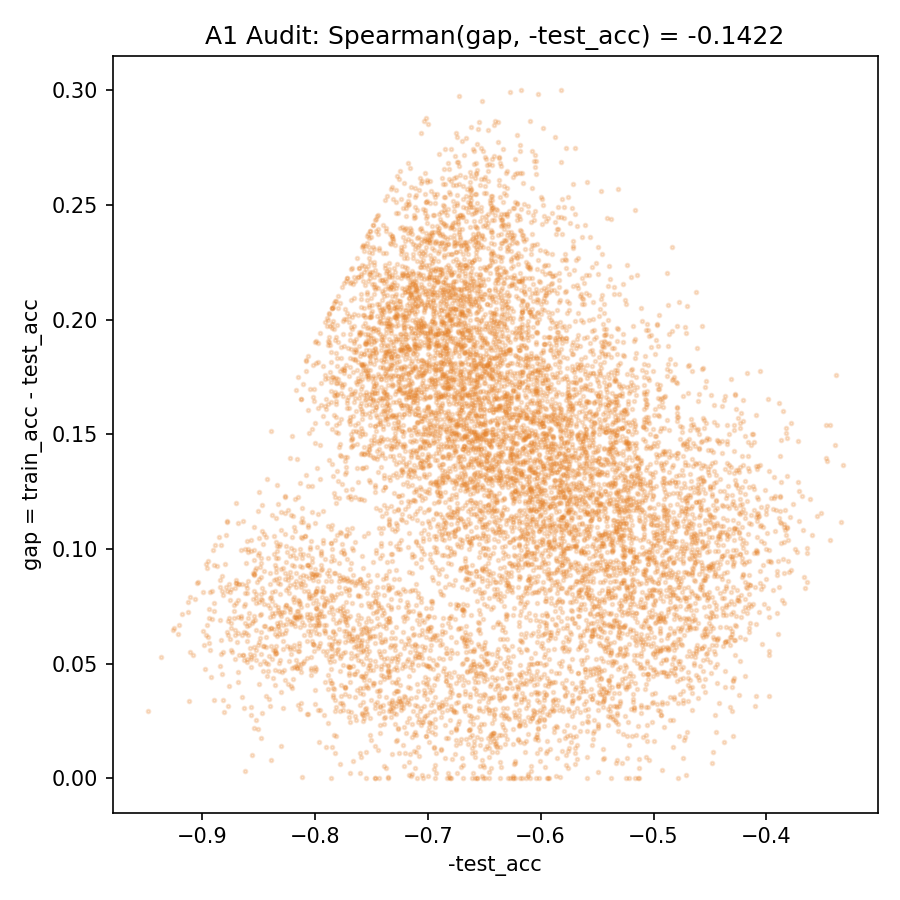
\includegraphics[width=0.9\columnwidth]{figures/a1_audit_scatter}
\caption{A1 audit scatter: gap vs.\ $-$test\_acc. Spearman $= -0.142$, confirming independence.}
\label{fig:a1_audit}
\end{figure}

\begin{figure}[h]
\centering
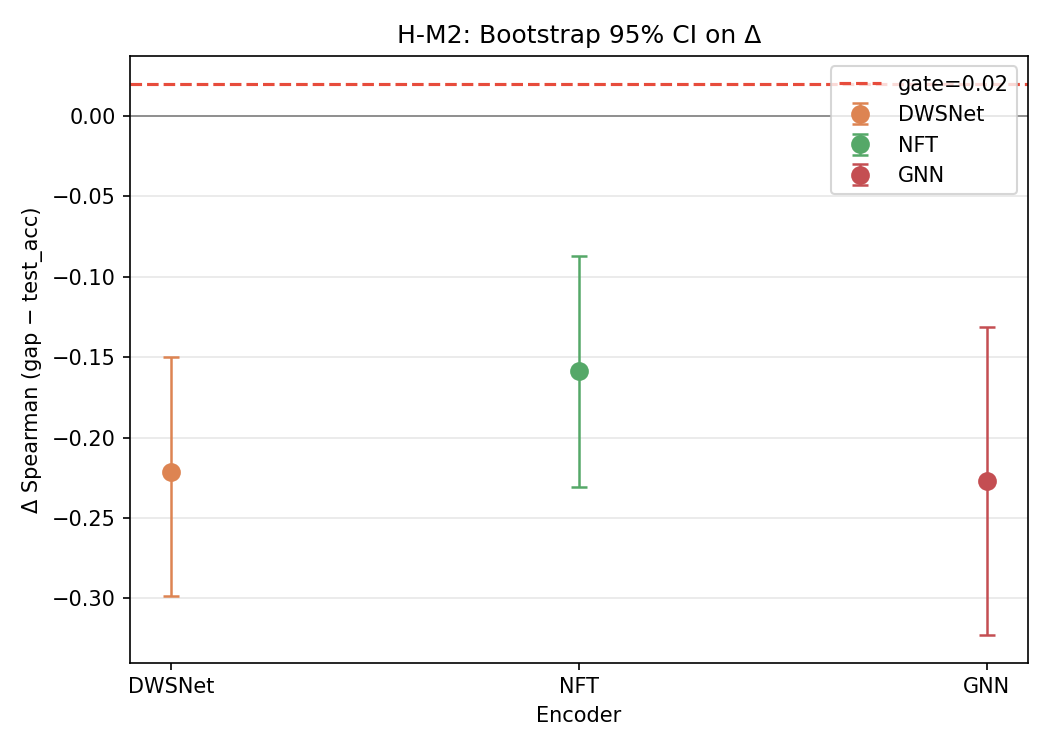
\includegraphics[width=0.9\columnwidth]{figures/fig5_bootstrap_ci}
\caption{Bootstrap 95\% confidence intervals for all Spearman estimates.}
\label{fig:bootstrap_ci}
\end{figure}

\begin{figure}[h]
\centering
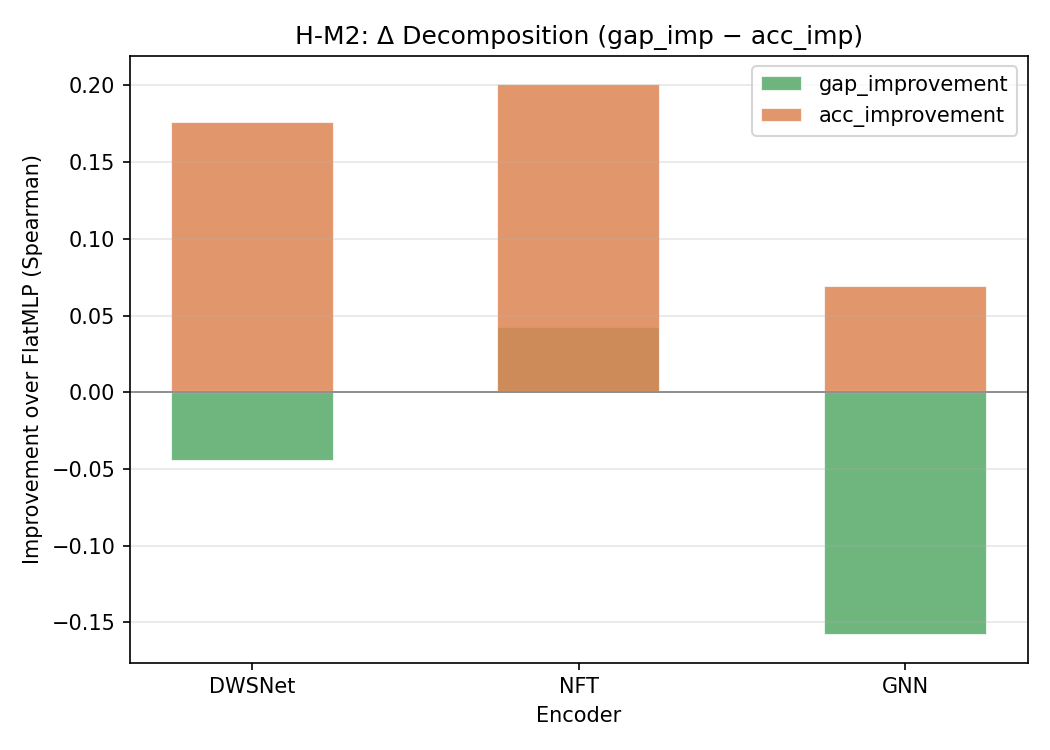
\includegraphics[width=0.9\columnwidth]{figures/fig3_delta_decomposition}
\caption{$\Delta$ decomposition: gap improvement vs.\ test\_acc improvement over FlatMLP for each equivariant encoder.}
\label{fig:delta_decomp}
\end{figure}

\begin{figure}[h]
\centering
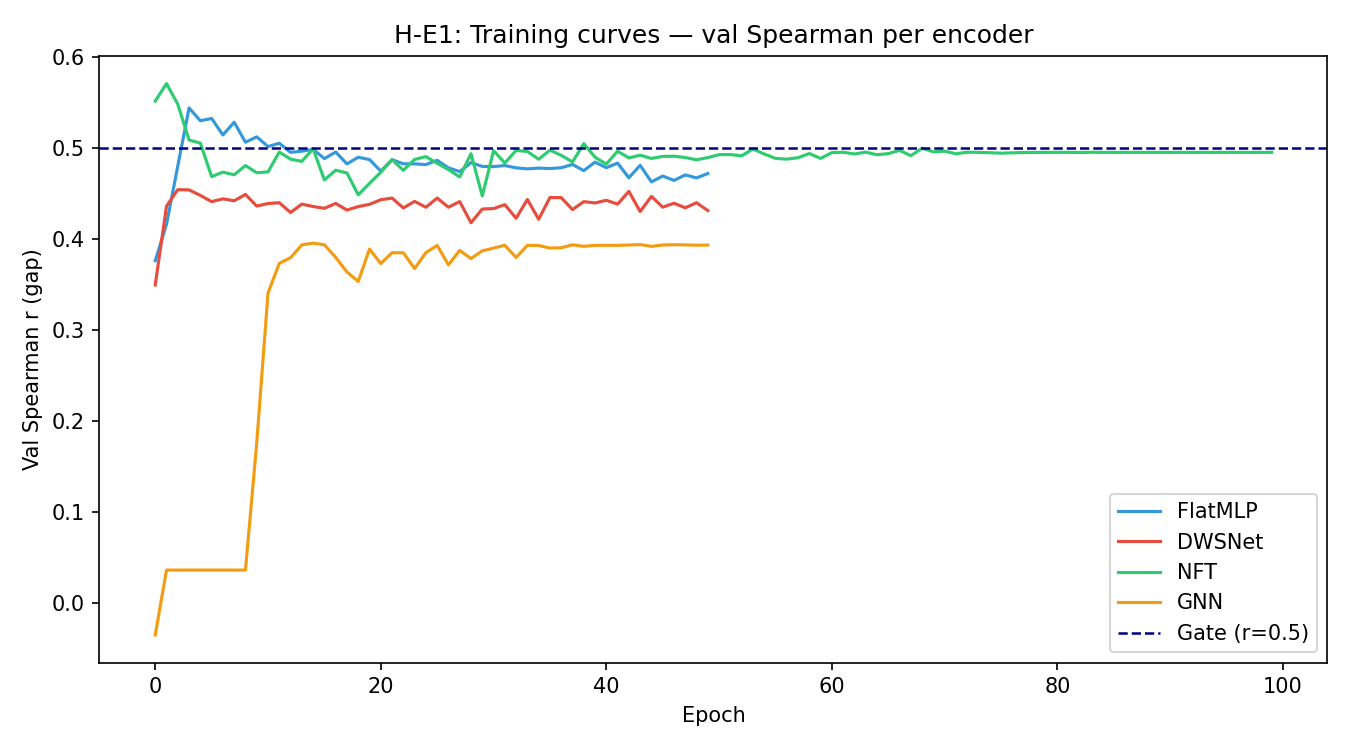
\includegraphics[width=0.9\columnwidth]{figures/training_curves}
\caption{Training curves (validation Spearman vs.\ epoch) for all encoders on both targets.}
\label{fig:training_curves}
\end{figure}


\end{document}
